As the application launches, the first screen the user sees, in both the Google Glass version and the smartphone version, is the camera screen. The user must, in order to proceed further within the application, scan a QR code. Scanning a QR code is done by positioning the device's camera such that the QR code can be seen on screen, as seen in Figure~\ref{glassDemoQR}. The user does not need to press any shutter button as the application automatically recognises the QR code pattern if seen on screen.%, as seen in Figure~\ref{}. The reasoning behind 

%	\begin{figure}[ht!]
%		\centering
%		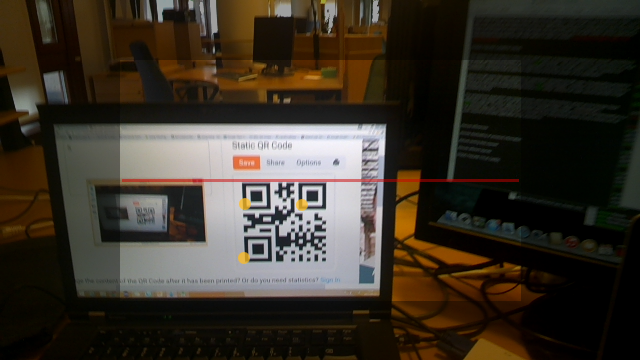
\includegraphics[width=110mm]{images/demo/qrCode}
%		\caption{todo bild behöver uppdateras}
%		\label{glassDemoQR}
%	\end{figure}
	
	\begin{figure}[ht!]
		\centering
    		\subfloat[The Google Glass application]{{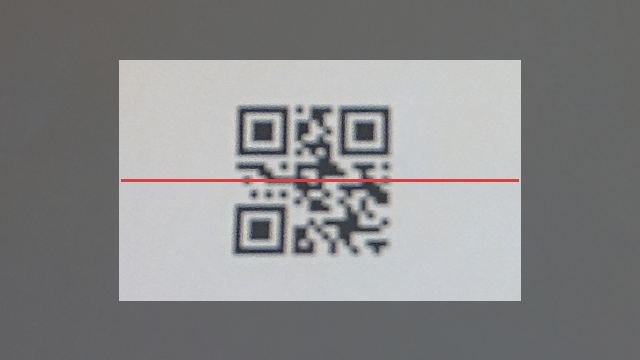
\includegraphics[width=70mm]{images/demo/qrCodeNew}}}
   		 \qquad
		\subfloat[The smartphone application.]{{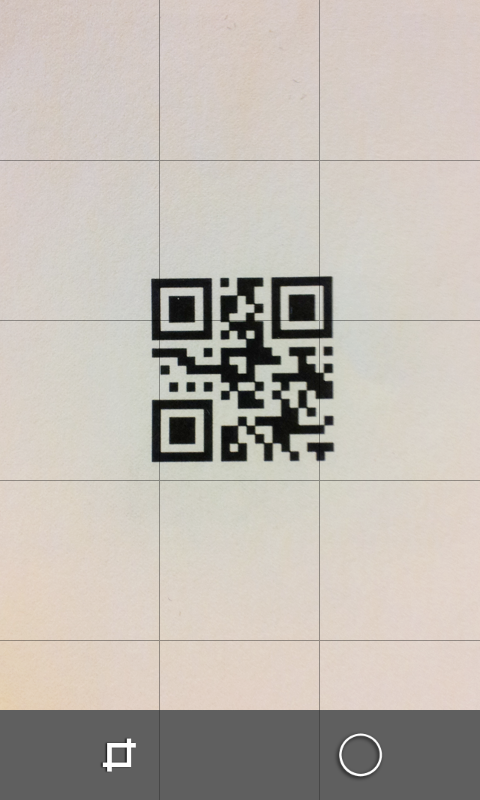
\includegraphics[width=70mm]{images/demo/smartphone/qrCodeNew}}}
   		 \qquad
		\caption{The application is scanning a QR code.}
		\label{glassDemoQR}
	\end{figure}

The reason for not providing a menu on the start screen or even requiring the user to press a shutter button is because the application should be simple, easy to use and focus on what is important. Since the the first step when using the application is to scan a QR code in order to receive the necessary information on the specific product, the scanning is also the main focus on the first screen of the application.

When the QR code has been scanned the application decodes the QR code. The decoding process is handled by the Zebra Crossing (ZXing) library~\cite{zxing}. ZXing is an open source barcode image processing library which uses the default QR code reader installed on the device.

The smartphone application was based directly on the ZXing library, where as the Google Glass application was based on a port of the ZXing library to Google Glass, called ``BardcodeEye''~\cite{barcodeEye}. The main difference between ZXing and BarcodeEye is the fact that BarcodeEye is an example application ready to be run on Google Glass, in contrast to the ZXing library which is only a library and as such needs to be attached to a runnable application.

The BarcodeEye application for Google Glass is however a bare bone application, used as an example and introduction as to how ZXing may be implemented in an application for Google Glass. BarcodeEye displays the decoded information from the QR code and also gives the user the option to search the internet using the information previously decoded from the QR code.

As the QR code is meant to encode only a product ID, and the application will then use the ID to download the product information (rather than having all of the instructions encoded directly in the QR code), the BarcodeEye application had to be modified. The first modification was on the graphical layout of the BarcodeEye application. The change of layout was mostly done due to the fact that the BarcodeEye application only displayed plain text, not taking in to account for instance a mix of image and text.

In order to display information BarcodeEye used the deprecated class \texttt{Card}, as seen in Listing~\ref{listingDeprecated}. The application now instead uses the \texttt{CardBuilder} class, as seen in Listing~\ref{listingRecommended}, as recommended by Google~\cite{googleCard}. The \texttt{CardBuilder} class allows users to input a desired layout style as an argument to the constructor of the \texttt{CardBuilder} class. With the \texttt{Card} class developers could in a separate method call set where on the card the image would appear. For instance, in order to create a columns card, as seen in Figure~\ref{glassDemoComponentColumn}, the code would look as the code in Listing~\ref{listingDeprecated}. Using the recommended \texttt{CardBuilder} class instead would look as the code in Listing~\ref{listingRecommended}. With \texttt{CardBuilder} developers can now use default layouts, enabling more consistent application design across Google Glass applications. If a developers wishes to use a custom layout instead, the developer can simply use the custom layout as input to the \texttt{CardBuilder} constructor instead.

\begin{lstlisting}[language=Java, caption={Instancing of the deprecated class Card}, label=listingDeprecated]
Card card = new Card(context);
card.setImageLayout(Card.ImageLayout.LEFT);
\end{lstlisting}

\begin{lstlisting}[language=Java, caption={Instancing of the recommended class CardBuilder}, label=listingRecommended]
CardBuilder cardBuilder = new CardBuilder(context, CardBuilder.Layout.COLUMNS);
\end{lstlisting}

Since the smartphone application also used the ZXing library, but without any pre-existing application, no changes similar to those done to the Google Glass application had to be done for the smartphone application. Instead the smartphone application was built from the ground up to make use of the ZXing library's functionality, similar to how the ZXing library was integrated in the base Google Glass application.

%The Google Glass application and the smartphone application are similar in how they are built, as seen in Figure~\ref{uml}, which shows a UML diagram over the slide view part of the respective applications.

%[TODO UML DIAGRAM ref(uml)]

%discuss differences (classes exclusive to the smartphone application and GG application respectivly)

%discuss downloading of product information

Having scanned and decoded a QR code the decoded information is then used to download information on the specific product. The downloaded information contains the product name, as well as necessary components and instructions for assembling the product. The components and instructions may be represented by text, images or both. 

The way the download process uses the decoded product ID is by concatenating the product ID with a URL adress, which connects to a database containing all necessary information regarding the specific product. The download process was done using a \texttt{AsyncTask}. An AsyncTask is a class which performs operations in the background on a different thread than the user interface, such that the user interface is not frozen when the download process is taking place~\cite{asyncTask}.

In the Google Glass application a loading bar pops up at the bottom of the screen when information is being downloaded, as seen in Figure~\ref{downloadLoading}~(a), indicating that the application is loading. Google calls the bar an ``Ìndeterminate Slider'', as the the class used in implementation is the same as for a regular Slider~\cite{indeterminateSlide}. A similar animation was added to the smartphone application. However, in contrast to the Google Glass application's loading bar the smartphone application instead displays a spinning wheel at the center of the screen, seen in Figure~\ref{downloadLoading}~(a), indicating that the application is loading. The spinning wheel is implemented by the \texttt{ProgressDialog} class~\cite{loadingWheel}.

in both cases of loading animation the animation is started in the \texttt{AsyncTask}, just before the download begins. The loading animation stops when the \texttt{AsyncTask} has finished downloading the product information.

%However, such a spinner was not implemented in the Google Glass application. The reason for not implementing such a download spinner in the Google Glass application was because the AsyncTask, in order to display anything during the execution of the AsyncTask, requires access to a \texttt{Context} instance. A context comes from an activity in the android application, but in the Google Glass application the download process i taking place in between the scanning activity and the presenting activity. As such, the loading spinner 

	\begin{figure}[ht!]
		\centering
    		\subfloat[The Google Glass application]{{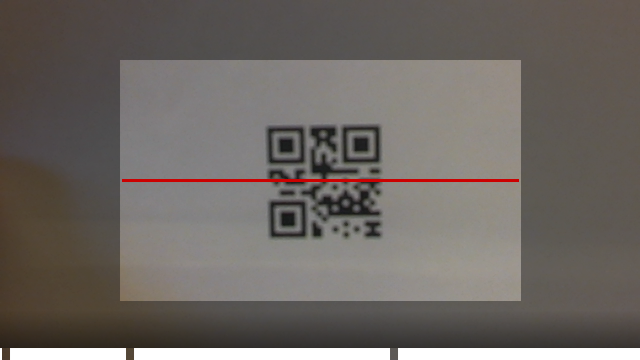
\includegraphics[width=70mm]{images/demo/loadingBar}}}
   		 \qquad
		\subfloat[The smartphone application.]{{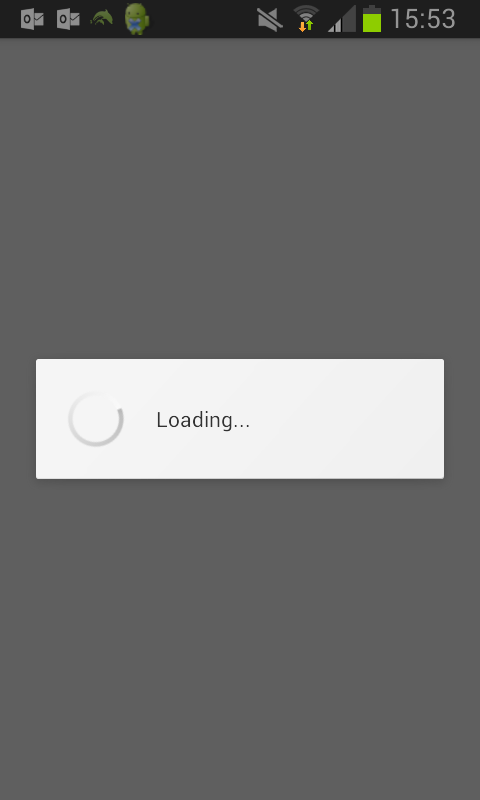
\includegraphics[width=70mm]{images/demo/smartphone/loadingSpinner}}}
   		 \qquad
		\caption{The loading screens.}
		\label{downloadLoading}
	\end{figure}

The download process also includes creating and initialise an instance of the \texttt{Products} class. The instance contains the name of the product and an image of the product as the product will look when the user is done assembling all the components (the existence of an image is dependent of whether there was an image of the product stored in the database or not).

The Products class instance will also contain a list of components as well as a list of instructions. Both components and instructions are classes themselves. Similar to the \texttt{Products} class, instances of both the \texttt{Components} class and the \texttt{Instructions} class will contain a string and potentially an image, depending on wether there is an image stored in the database or not. In the case of components the string attribute will contain the name of the component, in contrast to instances of the \texttt{Instructions} class where the string instead will contain the instruction itself.

When the downloaded information is being displayed, the first screen the user sees contains the product name as well as an image of the product (if an image existed in the database). In the example case, lego parts are to be assembled in order to construct the so called ``Space Pirate'', seen in Figure~\ref{glassDemoRaw}.

	\begin{figure}[ht!]
		\centering
		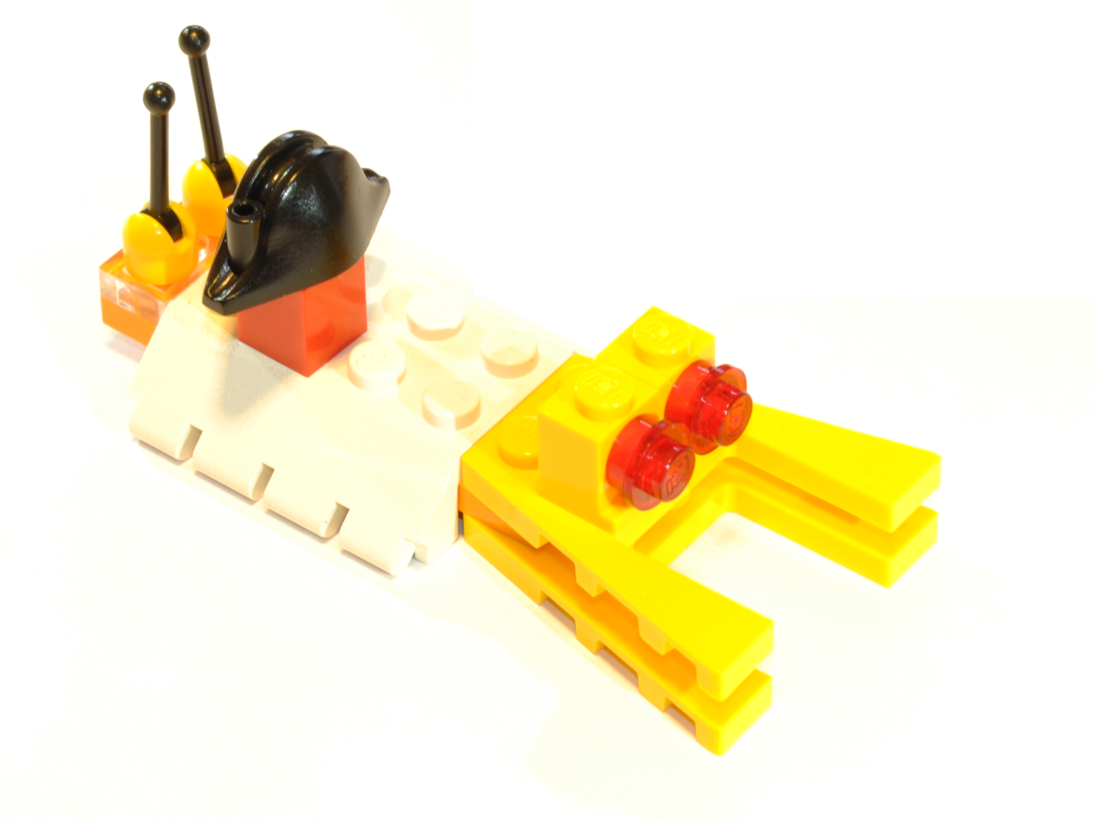
\includegraphics[width=90mm]{images/rawImages/BILD_6}
		\caption{The product.}
		\label{glassDemoRaw}
	\end{figure}

The first information the user sees displayed on screen after the QR code has been scanned and the information has been downloaded is the title page for the Space Pirate product, seen in Figure~\ref{glassDemoTitleCard}.

%	\begin{figure}[H]%ht!]
%		\centering
%		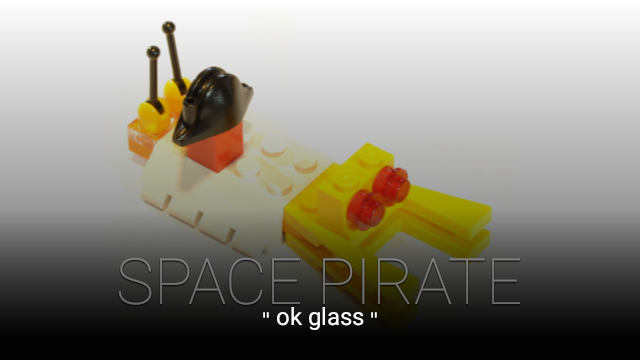
\includegraphics[width=110mm]{images/demo/titleCard}
%		\caption{The title card of the demo application.}
%		\label{glassDemoTitleCard}
%	\end{figure}
	
	\begin{figure}[ht!]
		\centering
    		\subfloat[The Google Glass application]{{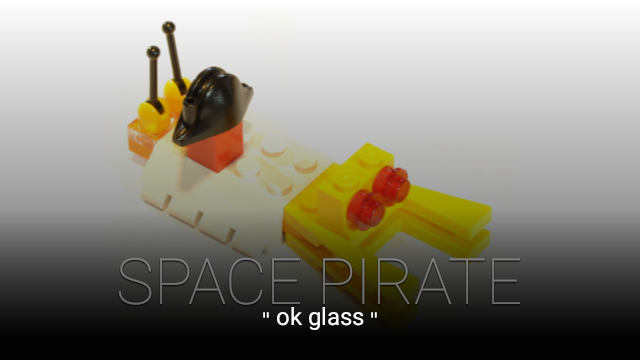
\includegraphics[width=70mm]{images/demo/titleCard}}}
   		 \qquad
		\subfloat[The smartphone application.]{{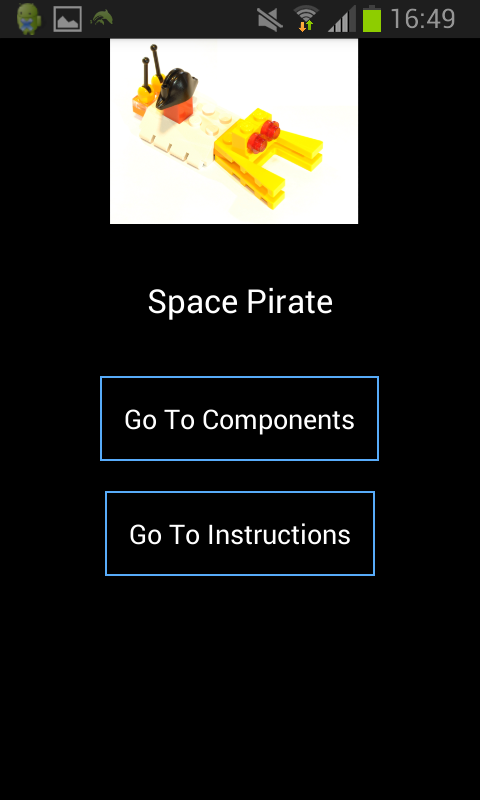
\includegraphics[width=70mm]{images/demo/smartphone/titleCard}}}
   		 \qquad
		\caption{The title card of the demo application.}
		\label{glassDemoTitleCard}
	\end{figure}
	
The next slide in line after the title slide is the first slide containing information on the components necessary for constructing the specific product. Each component has their own slide as the component may contain an image in complement to the name of the component. Examples of a component described in only text can been seen in Figure~\ref{glassDemoComponentText} and examples of when the component has been described with both text and image can be seen in Figure~\ref{glassDemoComponentColumn}.

As seen in Figure~\ref{glassDemoComponentText} the text in the Google Glass application is larger than the text in the smartphone application. The difference in size is due to the automatic scaling in the Google Glass application. If the text in the Google Glass application where to cover the entire screen the text size would automatically be downscaled. In the smartphone application, however, the text is always of the same size. The size of the text in the smartphone application was set to \texttt{MEDIUM} which is one of the three different default sizes of text used in android applications. The footer text, which in Figure~\ref{glassDemoComponentText} says ``Components'', as well as ``1/4'', is of the default size \texttt{SMALL}. In Figure~\ref{glassDemoTitleCard} the size of the product name text is of the default size \texttt{LARGE}. The reason behind the choice of the different text sizes is to keep the smartphone application similar to the Google Glass application, making the comparison of the two version easier.
%	\begin{figure}[H]%ht!]
%		\centering
%		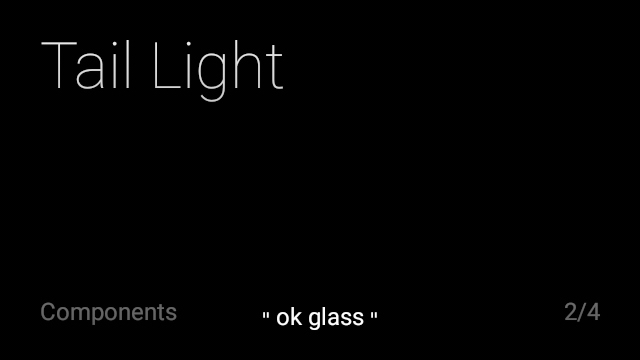
\includegraphics[width=110mm]{images/demo/componentText}
%		\caption{A component slide from the demo application.}
%		\label{glassDemoComponentText}
%	\end{figure}

		\begin{figure}[ht!]
		\centering
    		\subfloat[The Google Glass application]{{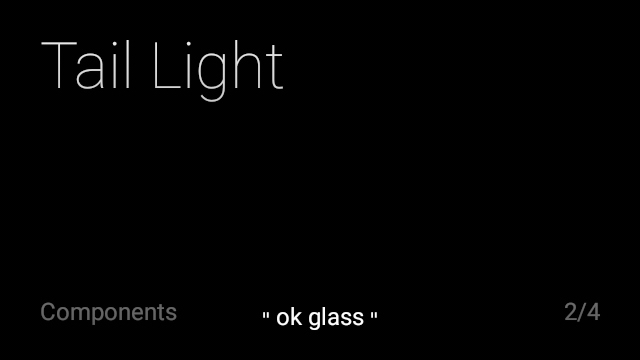
\includegraphics[width=70mm]{images/demo/componentText}}}
   		 \qquad
		\subfloat[The smartphone application.]{{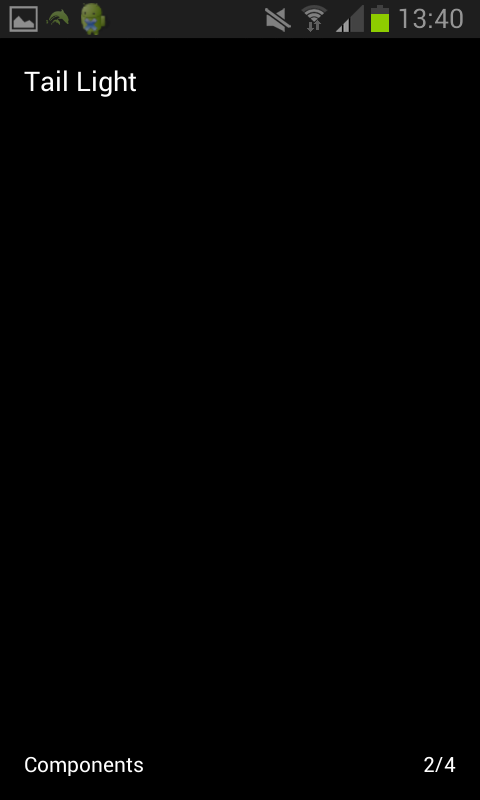
\includegraphics[width=70mm]{images/demo/smartphone/componentText}}}
   		 \qquad
		\caption{A component slide from the demo application.}
		\label{glassDemoComponentText}
	\end{figure}

%	\begin{figure}[H]%ht!]
%		\centering
%		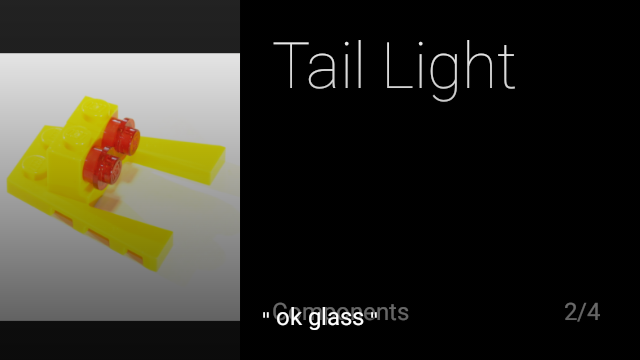
\includegraphics[width=110mm]{images/demo/columnImage}
%		\caption{A component slide from the demo application.}
%		\label{glassDemoComponentColumn}
%	\end{figure}
	
	\begin{figure}[ht!]
		\centering
    		\subfloat[The Google Glass application]{{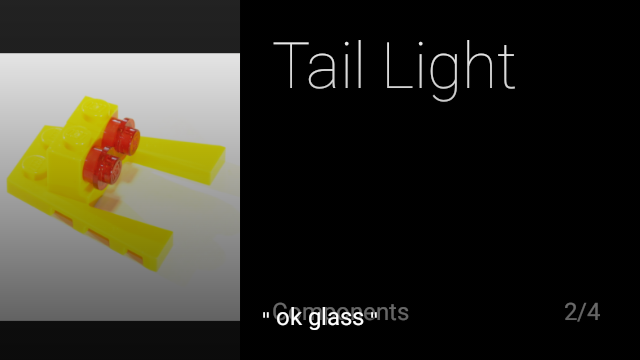
\includegraphics[width=70mm]{images/demo/columnImage}}}
   		 \qquad
		\subfloat[The smartphone application.]{{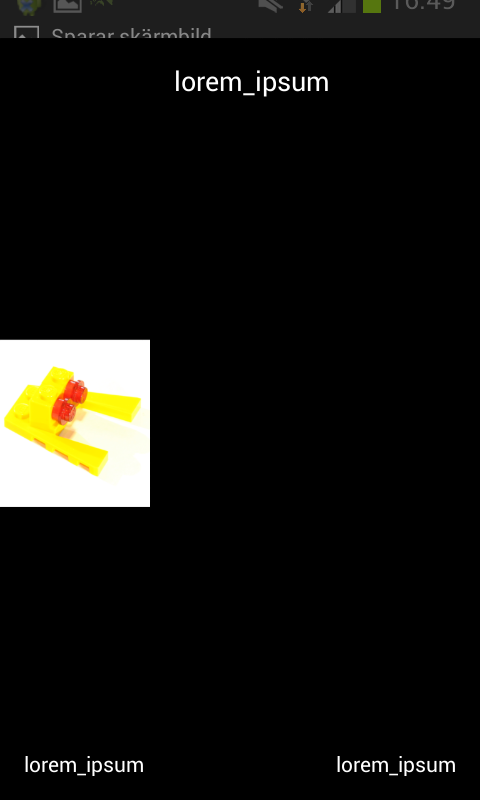
\includegraphics[width=70mm]{images/demo/smartphone/columnImage}}}
   		 \qquad
		\caption{A component slide from the demo application.}
		\label{glassDemoComponentColumn}
	\end{figure}

%	\begin{figure}[H]%ht!]
%		\centering
%		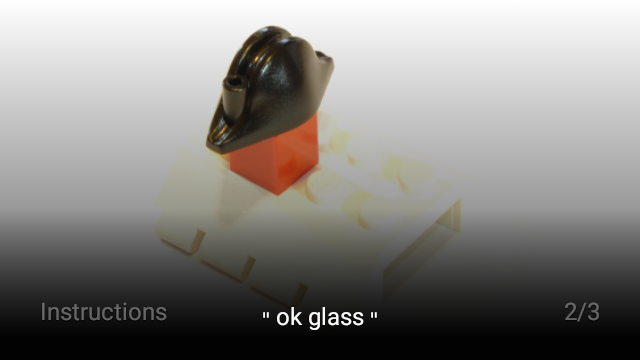
\includegraphics[width=110mm]{images/demo/instructionImage}
%		\caption{An instruction slide from the demo application.}
%		\label{glassDemoInstructionImage}
%	\end{figure}

The card design used for the component slide containing only text, seen in Figure~\ref{glassDemoComponentText}, is the predefined \texttt{TEXT} layout, used in similar fashion to how the title card design was specified in Listing~\ref{listingRecommended}. A component slide may also contain an image as complement to text. The card design used for the component slide containing both text and image, seen in Figure~\ref{glassDemoComponentColumn} is the predefined \texttt{COLUMNS} layout, used in similar fashion to how the title card design was specified in Listing~\ref{listingRecommended}

After all the component slides comes the instruction slides. These slides may also contain either only text or both text and an image, and these layouts are specified the same way as the component slides. However, an instruction slide may also consist of only an image, and no text at all. The reason for giving an image exclusive layout as a possible card layout for an instruction slide is because an instruction may be best described with an image. Describing the same instruction in text may take up more slides than the image, as the image will only take up one slide. A slide containing only an image and no text will also mean that the image will be scaled larger than when using both text and an image. As such more detail can be shown and users may get a better understanding for how the components should be assembled.

As seen in Figure~\ref{glassDemoInstructionImage}, one instruction is described with only an image and no text. Since the placement of the components are important, and potentially hard to specify in text, an image may describe the placement better. Note also that the smartphone application still has room for text. Potentially the image in the smartphone application could be expanded, for instance by giving the user the ability to zoom by pinch. However, such a feature does not exist.

	\begin{figure}[ht!]
		\centering
    		\subfloat[The Google Glass application]{{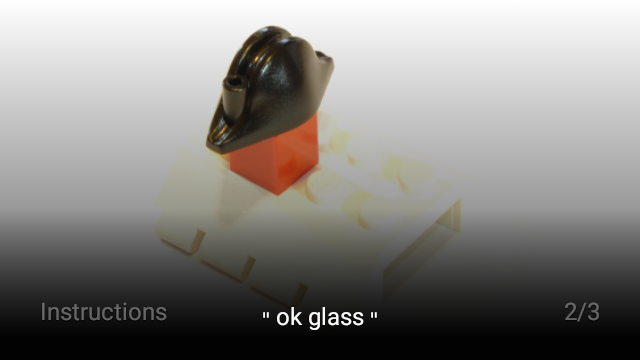
\includegraphics[width=70mm]{images/demo/instructionImage}}}
   		 \qquad
		\subfloat[The smartphone application.]{{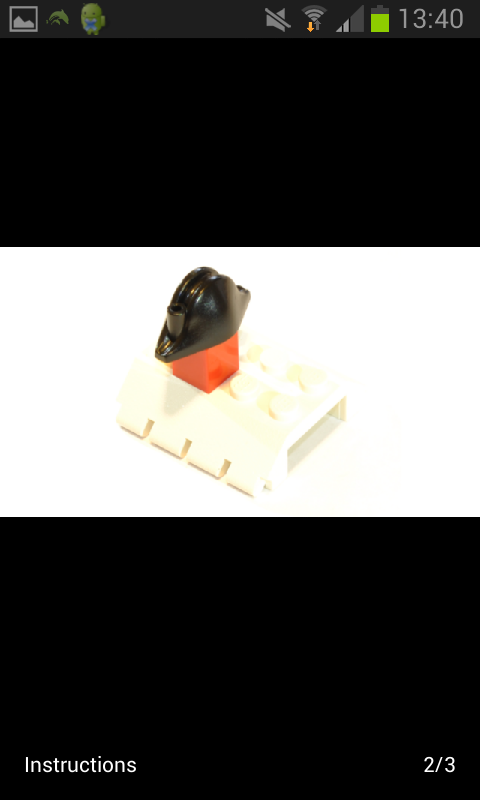
\includegraphics[width=70mm]{images/demo/smartphone/instructionImage}}}
   		 \qquad
		\caption{An instruction slide from the demo application.}
		\label{glassDemoInstructionImage}
	\end{figure}
	
The Google Glass application may be controlled by swiping across the Google Glass touchpad, but the Google Glass application may also be controlled using voice commands. The voice commands can be used as simple replacement for the touchpad, where users may swipe cards both backwards and forwards. However, using voice commands users may also ``jump'' in the application. By for instance saying ``ok glass, show components'' the application jumps to the first component slide, regardless of which slide the user is currently viewing. If the user is currently already viewing the first component slide nothing will happen. The voice command menu of the Google Glass application can be seen in Figure~\ref{glassDemoVoiceCommand}. Although the smartphone application does not have any voice command features the title slide contains buttons, as seen in Figure~\ref{glassDemoTitleCard}~(b) giving the user the ability to skip straight to the instructions is so desired.
	
	\begin{figure}[ht!]
		\centering
		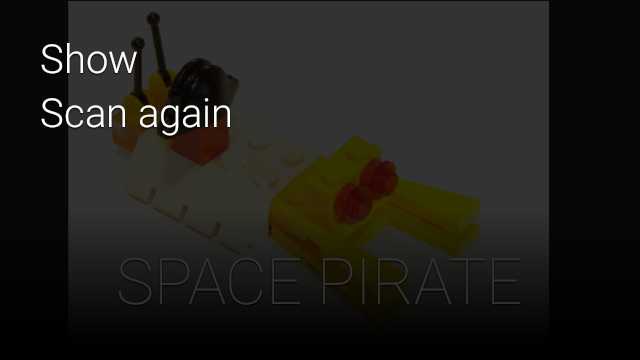
\includegraphics[width=90mm]{images/demo/voiceCommand1}
		\caption{The voice command menu in the demo application.}
		\label{glassDemoVoiceCommand}
	\end{figure}

%discuss sorting into classes

%discuss different layouts